% Options for packages loaded elsewhere
\PassOptionsToPackage{unicode}{hyperref}
\PassOptionsToPackage{hyphens}{url}
\documentclass[
  12pt,
]{article}
\usepackage{xcolor}
\usepackage[margin=2.5cm]{geometry}
\usepackage{amsmath,amssymb}
\setcounter{secnumdepth}{5}
\usepackage{iftex}
\ifPDFTeX
  \usepackage[T1]{fontenc}
  \usepackage[utf8]{inputenc}
  \usepackage{textcomp} % provide euro and other symbols
\else % if luatex or xetex
  \usepackage{unicode-math} % this also loads fontspec
  \defaultfontfeatures{Scale=MatchLowercase}
  \defaultfontfeatures[\rmfamily]{Ligatures=TeX,Scale=1}
\fi
\usepackage{lmodern}
\ifPDFTeX\else
  % xetex/luatex font selection
  \setmainfont[]{Times New Roman}
\fi
% Use upquote if available, for straight quotes in verbatim environments
\IfFileExists{upquote.sty}{\usepackage{upquote}}{}
\IfFileExists{microtype.sty}{% use microtype if available
  \usepackage[]{microtype}
  \UseMicrotypeSet[protrusion]{basicmath} % disable protrusion for tt fonts
}{}
\makeatletter
\@ifundefined{KOMAClassName}{% if non-KOMA class
  \IfFileExists{parskip.sty}{%
    \usepackage{parskip}
  }{% else
    \setlength{\parindent}{0pt}
    \setlength{\parskip}{6pt plus 2pt minus 1pt}}
}{% if KOMA class
  \KOMAoptions{parskip=half}}
\makeatother
\usepackage{color}
\usepackage{fancyvrb}
\newcommand{\VerbBar}{|}
\newcommand{\VERB}{\Verb[commandchars=\\\{\}]}
\DefineVerbatimEnvironment{Highlighting}{Verbatim}{commandchars=\\\{\}}
% Add ',fontsize=\small' for more characters per line
\usepackage{framed}
\definecolor{shadecolor}{RGB}{248,248,248}
\newenvironment{Shaded}{\begin{snugshade}}{\end{snugshade}}
\newcommand{\AlertTok}[1]{\textcolor[rgb]{0.94,0.16,0.16}{#1}}
\newcommand{\AnnotationTok}[1]{\textcolor[rgb]{0.56,0.35,0.01}{\textbf{\textit{#1}}}}
\newcommand{\AttributeTok}[1]{\textcolor[rgb]{0.13,0.29,0.53}{#1}}
\newcommand{\BaseNTok}[1]{\textcolor[rgb]{0.00,0.00,0.81}{#1}}
\newcommand{\BuiltInTok}[1]{#1}
\newcommand{\CharTok}[1]{\textcolor[rgb]{0.31,0.60,0.02}{#1}}
\newcommand{\CommentTok}[1]{\textcolor[rgb]{0.56,0.35,0.01}{\textit{#1}}}
\newcommand{\CommentVarTok}[1]{\textcolor[rgb]{0.56,0.35,0.01}{\textbf{\textit{#1}}}}
\newcommand{\ConstantTok}[1]{\textcolor[rgb]{0.56,0.35,0.01}{#1}}
\newcommand{\ControlFlowTok}[1]{\textcolor[rgb]{0.13,0.29,0.53}{\textbf{#1}}}
\newcommand{\DataTypeTok}[1]{\textcolor[rgb]{0.13,0.29,0.53}{#1}}
\newcommand{\DecValTok}[1]{\textcolor[rgb]{0.00,0.00,0.81}{#1}}
\newcommand{\DocumentationTok}[1]{\textcolor[rgb]{0.56,0.35,0.01}{\textbf{\textit{#1}}}}
\newcommand{\ErrorTok}[1]{\textcolor[rgb]{0.64,0.00,0.00}{\textbf{#1}}}
\newcommand{\ExtensionTok}[1]{#1}
\newcommand{\FloatTok}[1]{\textcolor[rgb]{0.00,0.00,0.81}{#1}}
\newcommand{\FunctionTok}[1]{\textcolor[rgb]{0.13,0.29,0.53}{\textbf{#1}}}
\newcommand{\ImportTok}[1]{#1}
\newcommand{\InformationTok}[1]{\textcolor[rgb]{0.56,0.35,0.01}{\textbf{\textit{#1}}}}
\newcommand{\KeywordTok}[1]{\textcolor[rgb]{0.13,0.29,0.53}{\textbf{#1}}}
\newcommand{\NormalTok}[1]{#1}
\newcommand{\OperatorTok}[1]{\textcolor[rgb]{0.81,0.36,0.00}{\textbf{#1}}}
\newcommand{\OtherTok}[1]{\textcolor[rgb]{0.56,0.35,0.01}{#1}}
\newcommand{\PreprocessorTok}[1]{\textcolor[rgb]{0.56,0.35,0.01}{\textit{#1}}}
\newcommand{\RegionMarkerTok}[1]{#1}
\newcommand{\SpecialCharTok}[1]{\textcolor[rgb]{0.81,0.36,0.00}{\textbf{#1}}}
\newcommand{\SpecialStringTok}[1]{\textcolor[rgb]{0.31,0.60,0.02}{#1}}
\newcommand{\StringTok}[1]{\textcolor[rgb]{0.31,0.60,0.02}{#1}}
\newcommand{\VariableTok}[1]{\textcolor[rgb]{0.00,0.00,0.00}{#1}}
\newcommand{\VerbatimStringTok}[1]{\textcolor[rgb]{0.31,0.60,0.02}{#1}}
\newcommand{\WarningTok}[1]{\textcolor[rgb]{0.56,0.35,0.01}{\textbf{\textit{#1}}}}
\usepackage{longtable,booktabs,array}
\usepackage{calc} % for calculating minipage widths
% Correct order of tables after \paragraph or \subparagraph
\usepackage{etoolbox}
\makeatletter
\patchcmd\longtable{\par}{\if@noskipsec\mbox{}\fi\par}{}{}
\makeatother
% Allow footnotes in longtable head/foot
\IfFileExists{footnotehyper.sty}{\usepackage{footnotehyper}}{\usepackage{footnote}}
\makesavenoteenv{longtable}
\usepackage{graphicx}
\makeatletter
\newsavebox\pandoc@box
\newcommand*\pandocbounded[1]{% scales image to fit in text height/width
  \sbox\pandoc@box{#1}%
  \Gscale@div\@tempa{\textheight}{\dimexpr\ht\pandoc@box+\dp\pandoc@box\relax}%
  \Gscale@div\@tempb{\linewidth}{\wd\pandoc@box}%
  \ifdim\@tempb\p@<\@tempa\p@\let\@tempa\@tempb\fi% select the smaller of both
  \ifdim\@tempa\p@<\p@\scalebox{\@tempa}{\usebox\pandoc@box}%
  \else\usebox{\pandoc@box}%
  \fi%
}
% Set default figure placement to htbp
\def\fps@figure{htbp}
\makeatother
% definitions for citeproc citations
\NewDocumentCommand\citeproctext{}{}
\NewDocumentCommand\citeproc{mm}{%
  \begingroup\def\citeproctext{#2}\cite{#1}\endgroup}
\makeatletter
 % allow citations to break across lines
 \let\@cite@ofmt\@firstofone
 % avoid brackets around text for \cite:
 \def\@biblabel#1{}
 \def\@cite#1#2{{#1\if@tempswa , #2\fi}}
\makeatother
\newlength{\cslhangindent}
\setlength{\cslhangindent}{1.5em}
\newlength{\csllabelwidth}
\setlength{\csllabelwidth}{3em}
\newenvironment{CSLReferences}[2] % #1 hanging-indent, #2 entry-spacing
 {\begin{list}{}{%
  \setlength{\itemindent}{0pt}
  \setlength{\leftmargin}{0pt}
  \setlength{\parsep}{0pt}
  % turn on hanging indent if param 1 is 1
  \ifodd #1
   \setlength{\leftmargin}{\cslhangindent}
   \setlength{\itemindent}{-1\cslhangindent}
  \fi
  % set entry spacing
  \setlength{\itemsep}{#2\baselineskip}}}
 {\end{list}}
\usepackage{calc}
\newcommand{\CSLBlock}[1]{\hfill\break\parbox[t]{\linewidth}{\strut\ignorespaces#1\strut}}
\newcommand{\CSLLeftMargin}[1]{\parbox[t]{\csllabelwidth}{\strut#1\strut}}
\newcommand{\CSLRightInline}[1]{\parbox[t]{\linewidth - \csllabelwidth}{\strut#1\strut}}
\newcommand{\CSLIndent}[1]{\hspace{\cslhangindent}#1}
\setlength{\emergencystretch}{3em} % prevent overfull lines
\providecommand{\tightlist}{%
  \setlength{\itemsep}{0pt}\setlength{\parskip}{0pt}}
\usepackage{setspace}\doublespacing
\setstretch{1.5}
\usepackage{parskip}
\setlength{\parskip}{6pt}
\setlength{\parindent}{0pt}
\usepackage{float}
\newcommand{\argmin}{\mathop{\mathrm{argmin}}\limits}
\usepackage{booktabs}
\usepackage{caption}
\usepackage{longtable}
\usepackage{colortbl}
\usepackage{array}
\usepackage{anyfontsize}
\usepackage{multirow}
\usepackage{bookmark}
\IfFileExists{xurl.sty}{\usepackage{xurl}}{} % add URL line breaks if available
\urlstyle{same}
\hypersetup{
  pdftitle={The Foreign Policy Impact of Trade-Based Status Gains: Evidence from Brazil},
  pdfauthor={Author name omitted for peer review},
  hidelinks,
  pdfcreator={LaTeX via pandoc}}

\title{The Foreign Policy Impact of Trade-Based Status Gains: Evidence
from Brazil}
\author{Author name omitted for peer review\textsuperscript{}}
\date{2024-06-30}

\begin{document}
\maketitle
\begin{abstract}
\singlespacing Becoming the major trade partner of a country implies not
only increased trade ties but also a change in status. And yet, while
most research focuses on status anxiety or status-seeking behavior,
International Relations scholarship has largely overlooked the
consequences of an upward change in a state's standing. This paper
examines how a significant shift in a country's status can impact the
foreign policy alignment of another state. Using a Synthetic
Difference-in-Differences design, we investigate China's rise to become
Brazil's top trade partner in 2009, providing evidence on the effect of
status change on Brazil's foreign policy. We find that this shift led to
a 42\% reduction in the ideological distance between Brazil and China at
the United Nations General Assembly. To unpack the mechanism, an
NLP-based analysis of Brazil's main newspaper (2005-2013) reveals a
sharp increase in China-related salience, amplifying public and elite
attention to the new status quo. Together, these findings demonstrate
that status gains, once made salient by the media, can produce
measurable shifts in interstate alignment.
\end{abstract}

\pagebreak

\section{Introduction}\label{introduction}

``China overtakes US as Brazil's top trade partner''. Brazilian
newspapers ran similar headlines in 2009
(\citeproc{ref-rodrigues2009}{Rodrigues 2009};
\citeproc{ref-correio2009}{Correio Braziliense 2009};
\citeproc{ref-folha2009}{Folha de S.Paulo 2009}). Sensing the symbolic
weight of the milestone in Brazil, President Lula da Silva promptly
announced a high-profile trip to Beijing, flanked by an unusually large
business delegation. BBC ran a similar framing in 2021, when China
surpassed the United States as the EU's biggest trading partner
(\citeproc{ref-bbc2021}{BBC News 2021}). Understandably, media outlets
are interested in symbolic milestones when choosing their headlines.
Should a salient one-off rank reversal, rather than gradual accumulation
of trade, have lasting foreign-policy effects?

An extensive empirical literature shows that as a country's trade
dependence on China accumulates, its UN-voting distance from Beijing
tends to fall (\citeproc{ref-kastner_pearson2021}{Kastner and Pearson
2021}; \citeproc{ref-yan_zhou2021}{Yan and Zhou 2021};
\citeproc{ref-morgan_2019}{Morgan 2019};
\citeproc{ref-flores-macias_kreps2013}{Flores-Macías and Kreps 2013}),
the same being true for Brazil and China in particular
(\citeproc{ref-neto_malamud2015}{Neto and Malamud 2015};
\citeproc{ref-mouron_urdinez2014}{Mourón and Urdinez 2014}). Analysts
interpret this association in three ways: coercive leverage, i.e., China
rewards or punishes to shape votes (\citeproc{ref-tanner_2007}{Tanner
2007}; \citeproc{ref-reilly2013}{Reilly 2013}), interest redefinition
(growing commerce makes cooperation intrinsically valuable), and
societal pressure (business lobbies or public opinion pull leaders
toward Beijing). What these perspectives share is the assumption that
influence scales smoothly with commercial exposure: the more trade, the
more alignment --- no particular trade share or moment is distinguished
from another.

Research in cognitive psychology and political communication, by
contrast, emphasizes that actors respond disproportionately to salient
thresholds---events that break routine patterns and become focal in
media and politicians' agendas
(\citeproc{ref-baekgaard_etal2019}{Baekgaard et al. 2019};
\citeproc{ref-sheffer_etal2018}{Sheffer et al. 2018};
\citeproc{ref-edwards_wood1999}{Edwards and Wood 1999};
\citeproc{ref-mintz_geva1997}{Mintz and Geva 1997}). That is why
countries routinely look for marks and milestones such as the Olympics
to climb the ladder of status in world politics
(\citeproc{ref-mercer_2017}{Mercer 2017a}). While most of studies of
status emphasized how lacking status drives risk‑acceptant behaviour and
conflict, there is only anecdotal evidence that status yield tangible
diplomatic dividends (\citeproc{ref-gotz_2021}{Götz 2021}). As a result,
we know surprisingly little about the downstream effects when a state's
status actually rises.

Much has been studied about how China can impact the foreign policy of
small countries or highly dependent on the emerging superpower
(\citeproc{ref-yan_zhou2021}{Yan and Zhou 2021};
\citeproc{ref-chen_zhou2021}{Chen and Zhou 2021};
\citeproc{ref-aiyar_etal2024}{Aiyar, Malacrino, and Presbitero 2024}),
but studying the case of a developing country the size of Brazil is
important to advance the literature on the effect of such a change in
status beyond small countries. It is much easier for trade ties to
impact states with a high asymmetry. Another matter is a state that,
while still asymmetric in relation to China, is a regional power under
the direct sphere of influence of the US.

We investigate what are the political payoffs of an increase in status?
To answer it, we exploit a clear ``rank effect'': in 2009 China overtook
the United States as Brazil's top trading partner. We show that this
jump in economic status caused a 42\% reduction in Brazil's ideological
distance from China in UNGA votes.

We use a synthetic difference-in-differences approach to estimate the
causal effect of China becoming the first, as opposed to second, trade
partner for Brazil to estimate its causal effect on foreign policy
orientation, measured as the absolute distance in UNGA ideal point
estimation (\citeproc{ref-bailey_etal2017}{Bailey, Strezhnev, and Voeten
2017}) between Brazil and China over 1997-2015. WE complement this
analysis with usage of a Large Language Models analysis of Folha de São
Paulo headlines to demonstrate the media's role in publicizing, and thus
legitimizing, this newfound status. By foregrounding both the
quantitative effect and the salience channel, this study illuminates how
status gains reshape foreign policy. It also has broad implications for
the study of economic ties with an emerging power and the foreign policy
of countries. Similar status effects may be important for the impact of
other economic variables (such as Foreign Direct Investment, aid, and
loans) on the foreign policy of countries.

The rest of the paper is organized as follows. Next, we discuss the
importance of salience effects in the realm of trade effects and
political alignment. In the third section, we present our methodology,
data, and variables. Then, we present our empirical results. The fifth
section discusses some robustness checks. The sixth section highlights
evidence from the media, demonstrating the qualitative changes in
coverage that occurred when China surpassed the US in 2009. Finally, the
last section offers our concluding remarks and summarizes key takeaways.

\section{Trade and Political
Alignment}\label{trade-and-political-alignment}

The analysis of the impact on the foreign policy of Brazil of China
becoming its first trade partner builds on the literature on trade and
foreign policy, behavioral science and status theory in world politics.
Many studies have studies the effect of trade with China on foreign
policy. A strand of the literature argues that the trade effects are due
to China's coercive capacity to threaten countries into behaving in the
ways China wants (\citeproc{ref-tanner_2007}{Tanner 2007};
\citeproc{ref-reilly2013}{Reilly 2013}). Other studies suggest that
deepening economic ties create vested interests in which economic groups
would lobby on behalf of China due to their self-interest
(\citeproc{ref-kastner_pearson2021}{Kastner and Pearson 2021}). Another
argument is that economic integration can transform public and elite
opinion about China, either through soft power
(\citeproc{ref-morgan_2019}{Morgan 2019}) or by influencing the way
media report on China, thereby changing public perceptions
(\citeproc{ref-kastner_pearson2021}{Kastner and Pearson 2021}). Finally,
there is the dimension of structural power. China's diplomatic inroads
into Latin America opened up the possibility of more autonomy from the
US in the region (\citeproc{ref-struver_2014}{Struver 2014}). Schenoni
and Leiva (\citeproc{ref-schenoni_leiva2021}{2021}) argue that recent
changes in Brazilian foreign policy are the result of the pull of China
as a new great power, leading to what they term ``dual hegemony''.
According to the pioneering work by Neto
(\citeproc{ref-neto2011}{2011}), as Brazil became a more powerful
country, it could distance itself from the US. It is thus expected that
as China emerged as an important country, it would attract some
alignment of Brazilian foreign policy due to this power effect. Mourón
and Urdinez (\citeproc{ref-mouron_urdinez2014}{2014}) argued that the
power gap was the most important factor, and that it was true for the
broader South American countries: the smaller the power gap between a
country and the US, the less it aligned with the US at the UN.

Qualitative studies echo these findings. For instance,
(\citeproc{ref-guilhon2014}{Guilhon-Albuquerque 2014}) notes trade was
central to Brazil's foreign policy under Lula, while Vadell
(\citeproc{ref-vadell_2011}{2011}) shows China's diplomacy in South
America followed its economic interests.

These studies demonstrate that trade significantly impacts the foreign
policy of a country like Brazil. Some of the mechanisms proposed in the
literature for small states, such as coercion and threats, are not
applicable to Brazil. There is no evidence in the literature on the
relationship between the two countries of such measures by China
(\citeproc{ref-haibin_2010}{Haibin 2010};
\citeproc{ref-urdinez_2014}{Urdinez 2014};
\citeproc{ref-urdinez_etal2016}{Urdinez et al. 2016};
\citeproc{ref-brun_covarrubias2024}{Brun and Covarrubias 2024}), nor is
Brazil dependent on foreign aid or loans from China like smaller and
poorer countries.

Other studies have emphasized the reverse causal order. They contend
that complementarity of aligned national interests and shared identities
with the emerging discourse (\citeproc{ref-haibin_2010}{Haibin 2010})
and a revisionist stance towards the international order promoted more
trade links between countries
(\citeproc{ref-coutinho_rodriguez2024}{Coutinho and Rodriguez 2024}).
Numerous studies have found evidence that political alignment (or its
absence) can have a significant impact on trade flows. Countries that
bucked China's political preferences suffered subsequent trade declines
(\citeproc{ref-fuchs_klann2013}{Fuchs and Klann 2013}). Countries that
voted in support of the PRC (political alignment) in 1971 on the matters
of Taiwan enjoyed a surge in bilateral trade with China in the
immediately following year (\citeproc{ref-yan_zhou2021}{Yan and Zhou
2021}). In a more general quantitative study, Chen and Zhou
(\citeproc{ref-chen_zhou2021}{2021}) shows that a country tends to
import more from partners with whom it has friendly relations, which is
especially true for authoritarian states (such as China). Studies have
found a similar effect in other economic variables, such as foreign
direct investment (\citeproc{ref-aiyar_etal2024}{Aiyar, Malacrino, and
Presbitero 2024}).

The most similar study to ours in terms of causal ambition is the
pioneering quantitative study of Flores-Macías and Kreps
(\citeproc{ref-flores-macias_kreps2013}{2013}). They show that the more
countries trade with China, the more likely they are to side with China
on foreign policy, as measured by vote similarity at the UNGA. To
control for endogeneity, the authors employed two distinct approaches: a
fixed-effects model with lagged variables and two-stage least squares.
The first model is just wrong from a causal point of view, since one key
identification assumption in fixed effects models is no carry over
effects, which precludes the use of lagged dependent variable in the
regression (\citeproc{ref-blackwell_glynn2018}{Blackwell and Glynn
2018}; \citeproc{ref-imai_kim2019}{Imai and Kim 2019},
\citeproc{ref-imai_kim2021}{2021}). The instrument used in the latter
approach is the lagged energy production of a country. This variable,
however, fails to meet the exclusion restriction assumption needed for a
valid instrument, since energy production is, for example, related to
economic development, which may be a causal pathway from the instrument
to the outcome (political alignment). In general, it is very hard to
justify the exclusion restriction of instruments
(\citeproc{ref-mellon_2021}{Mellon 2021};
\citeproc{ref-bastardoz_2023}{Bastardoz et al. 2023};
\citeproc{ref-lal_etal2024}{Lal et al. 2024}), and this is no exception,
diminishing the credibility of the assumptions needed for causal
identification.

Current quantitative studies measure Brazil's foreign policy alignment
using UNGA vote similarity (\citeproc{ref-neto2011}{Neto 2011};
\citeproc{ref-flores-macias_kreps2013}{Flores-Macías and Kreps 2013};
\citeproc{ref-mouron_urdinez2014}{Mourón and Urdinez 2014}), but as
Bailey, Strezhnev, and Voeten (\citeproc{ref-bailey_etal2017}{2017})
shows, this is problematic: changes in agenda and policy can't be
separated. Bailey, Strezhnev, and Voeten
(\citeproc{ref-bailey_etal2017}{2017}) offers an improved metric using
ideal point estimation, enabling us to focus on genuine shifts in state
preference for this paper. By using their estimates, we measure only
state preference reorientation over time, which is crucial for the
paper's purpose.

While important, the idea that economic ties with China can alter the
perception and beliefs of political elites often overlooks how
decision-makers process information about economic relationships. Recent
work in cognitive and behavioral sciences suggests that the salience of
economic ties --- not just their material depth --- influences attention
and policy choices (\citeproc{ref-enke2024}{Enke 2024}). The role of
cues and heuristics in making foreign policy decisions has also been
discussed in international relations
(\citeproc{ref-jabarian_sartori2024}{Jabarian and Sartori 2024}).
Mechanisms include how redundant pieces of information nonetheless work
by shifting one's attention (\citeproc{ref-conlon2023}{Conlon 2023}),
whereby people neglect the correlated structure of information and treat
them as independent (\citeproc{ref-enke_zimermann2017}{Enke and
Zimmermann 2017}), or the importance of coarse categorization alongside
granular information by news organizations in helping people decide what
to pay attention to (\citeproc{ref-graeber_etal2025}{Graeber, Roth, and
Sammon 2025}).

A similar and older approach in International Relations is poliheuristic
theory (\citeproc{ref-mintz2004}{Mintz 2004},
\citeproc{ref-mintz_2005}{2005}). Due to information-processing
constraints, poliheuristic decision-making process is based on a non
exhaustive search in the sense that ``comparisons of policy options are
made within a (very) restrictive alternative set and attribute set''
(\citeproc{ref-mintz_geva1997}{Mintz and Geva 1997, 84}). Consequently,
policy dimensions or issues that attract attention may newly enter
decision-makers' consideration sets, even if they were previously
ignored.

The rank effect is not new in the political science literature and has
been documented in domestic politics before
(\citeproc{ref-anagol_fujiwara2016}{Anagol and Fujiwara 2016};
\citeproc{ref-folke_etal2016}{Folke, Persson, and Rickne 2016};
\citeproc{ref-granzier_etal2023}{Granzier, Pons, and Tricaud 2023}). It
helps to coordinate decisions and produce a bandwagon effect on voters
who want to vote for the winner. However, as far as we know, no one has
discussed rank effects in international politics, although they could be
just as likely to be real, as argued above. There is ample consensus
that status, understood sometimes as the position or rank in a
hierarchy, matters for world politics. Yet, there is no quantitative
study estimating how a positive status shock translates into concrete
policy concessions, voting behaviour, or political alignment.

The idea that status matters has been extensively studied in
international relations in the last fifteen years
(\citeproc{ref-dafoe_etal2014}{Dafoe, Renshon, and Huth 2014};
\citeproc{ref-miller_etal2015}{Miller et al. 2015};
\citeproc{ref-renshon_2016}{Renshon 2016};
\citeproc{ref-renshon_etal2018}{Renshon, Dafoe, and Huth 2018};
\citeproc{ref-duque_2018}{Duque 2018}; \citeproc{ref-parlar_2019}{Parlar
Dal 2019}; \citeproc{ref-gotz_2021}{Götz 2021};
\citeproc{ref-roren_2024}{Røren 2024}). A standard definition of status
in the literature is the ranking or relative standing of a state
(\citeproc{ref-macdonald_parent2021}{MacDonald and Parent 2021}). The
definition conflates a continuous measure (relative standing) with an
ordinal (thus, qualitative), namely, ranking. Being the first is
different from being the second. As the saying goes, the second can be
seen as the first loser. This ambiguity is problematic because it
obscures the difference between a qualitative change and a smooth
process. If we are talking about a continuous measure, it wouldn't
matter if the Chinese Olympic team was the first in the medal count
during the Beijing Olympics in 2008; what would matter is the number of
medals relative to other countries. However, if the rank is what is
important, then being the first at home is of ultimate importance. Our
argument is that being the first or the second is what people pay
attention to, due to information-processing constraints. As a result,
status should be viewed primarily as a qualitative concept, more
accurately captured by the notion of rank.

We draw on the notion of coarse categorization --- the tendency to rely
on broad, easily processed bins rather than fine-grained metrics when
confronting complexity (\citeproc{ref-graeber_etal2025}{Graeber, Roth,
and Sammon 2025}). We argue that China becoming Brazil's first trade
partner or overtaking the US are coarse categories that are often easier
to process or require less mental effort than granular information. Even
though decision-makers specialized in trade know the specific volume of
trade and how to put them into context, their job is easier when
communicating with parliamentary representatives, asking for funding for
an initiative, or even selling it from a marketing perspective. As a
result, we hypothesise that either directly or indirectly, such coarse
news is important in driving momentum to produce changes in the foreign
policy of a country like Brazil.

This contrasts with most theorizations of the link between trade and
foreign policy, which often overlook qualitative changes in the status
of a trade relationship. If decision-makers, business interests, and
public opinion are fully rational, then indeed what matters is the
level, or perhaps the speed, of change in the trade ties between
countries, or even the expectation of future gains. Thus, a rank change,
such as China becoming Brazil's top trade partner in 2009, overtaking
the US, constitutes a prime example of a change in status that serves as
a cue for policymakers to implement foreign policy changes. From the
perspective of a coarse categorization rule, Brazil's case provides the
ideal setting to test our theory, since being the first or second trade
partner is a coarse categorization of an otherwise continuous variable
observable by everyone. If there is no effect of such a rule, we
shouldn't observe an effect any different from other close years when
Brazil experienced trade growth with China. On the other hand, if status
matters and leaders look at coarse categories, then we should find an
effect exactly when the change occurs. The salience of China's new
status triggers the media, decision-makers, and business interests to
focus on China, leading to an alignment in foreign policy. It
facilitates the realization of the convergence of interests and the
adoption of a more favorable view towards the foreign partner, which is
self-serving.

The causal claim of the present paper can be summarized by the
simplified Directed Acyclic Graph (DAG)---a diagram that visually
represents assumed causal relationships---below. We represent the main
variables and proposed mechanisms, without any confounding variables, to
clarify the argument. We discuss the identification strategy in the next
section.

\begin{figure}
\centering
\pandocbounded{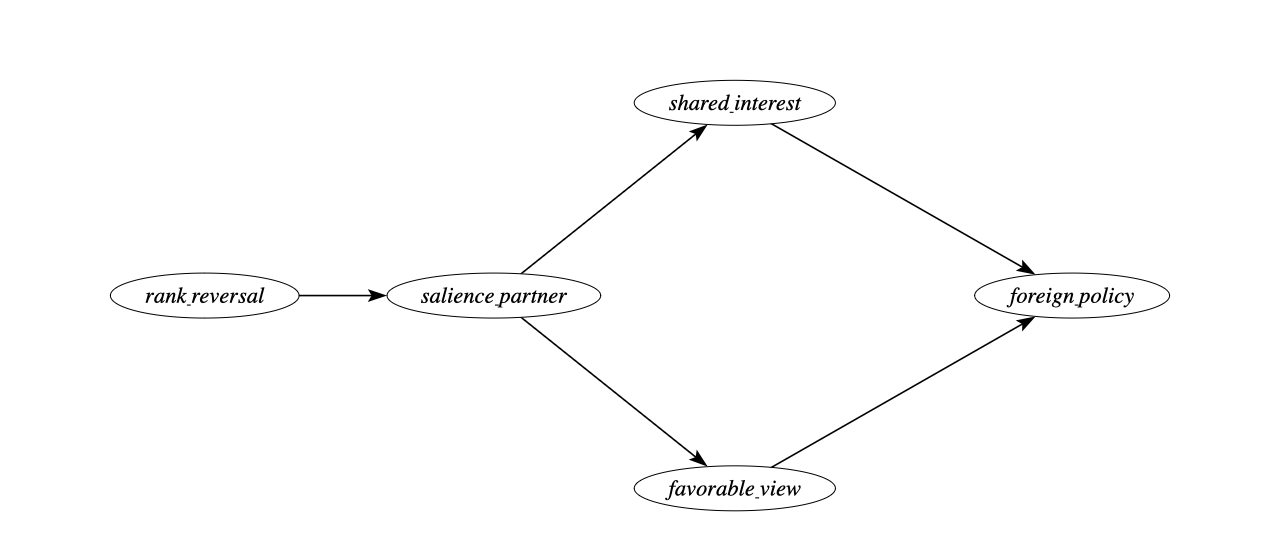
\includegraphics[keepaspectratio,alt={DAG of the causal relation}]{dag_trade_red.png}}
\caption{DAG of the causal relation}
\end{figure}

Our empirical evidence and research design cannot adjudicate between the
mechanisms of change in favorable views of China and the notion of
shared interests. That said, we provide credible evidence that a
salience effect exists and that it triggers a causal change in Brazil's
foreign policy.

\section{Methodology}\label{methodology}

We now explain how we will explore a discontinuity in Brazil's trade
partner shift---from the US to China---to estimate the (local) causal
effect of China's increased importance as Brazil's second-largest trade
partner. While we have a discontinuity, it might seem feasible to use a
Regression Discontinuity Design. However, our data are a time series
around a discontinuity, making this design inadequate.

A better alternative is the difference-in-differences (DiD) methodology.
The key identification assumption in DiD is the so-called parallel
trends assumption. This states that, absent the intervention, the
treated unit (Brazil) would behave just as the average of the control
group of countries. This assumption is not credible here. Many things
happened during this period---such as the 2008 economic crisis and its
subsequent effects---which undermine the credibility that countries
would respond in the same way to this shock. This leads to bias in
estimating the causal effect.

To avoid these problems, we employ the recently developed synthetic
difference-in-differences (SDiD) method
(\citeproc{ref-arkhangelsky_etal2021}{Arkhangelsky et al. 2021}). This
method combines the DiD estimator with the synthetic control method
(SCM), offering more flexibility than either method alone. DiD methods
are not well-suited for a single treated unit because they inflate the
standard error. SCM tries to match the pre-treatment trend in the
outcome using covariates to estimate the counterfactual outcome.
However, it compares the whole period before and after the intervention
and does not allow for unit fixed effects. This can cause bias,
especially if relevant time-invariant or slowly changing variables are
omitted. SDiD attempts to address both problems: improving the
adjustment for non-parallel trends in DiD and addressing the lack of
time weights and fixed effects in SCM. By combining the two methods,
SDiD enhances the ability to estimate causal effects. Similar to the SCM
model, we estimate the causal effect by comparing the post-treatment
behavior of the synthetic control and the treated unit, but with
additional robustness. The specific model is as follows:

Consider a complete panel\footnote{sometimes called a balanced panel. We
  prefer the term ``complete'' to avoid confusion with balancing of
  covariates, which is a standard analysis in causal studies}: \(N\)
countries measured over \(T\) years, the outcome variable for country
\(i\) in time \(t\) is \(Y_{it}\) and the binary treatment variable
\(D_{it} \in \{0,1\}\). Suppose also that the first
\(N_{\text{countries}}\) do not receive the treatment and the last
country \(N_{\text{Brazil}}\) does receive the treatment at \(t_0\). The
job is, like in SCM, to find weights \(\hat{w}^{\text{SDiD}}\) such that
before \(t_0\) treated and control countries match as closely as
possible, that is,
\(\sum_{i=1}^{\text{countries}} \hat{w}^{\text{SDiD}}Y_{it} \approx \sum_{i=1}^{\text{Brazil}} Y_{it}\),
for all \(t = 1, ..., t_0\). Unlike SCM, we do not stop here. We then
find \(\hat{\lambda}^{\text{SDiD}}_t\) to balance the time trend before
and after \(t_0\). Lastly, the average causal effect on the treated
\(\tau_{ATT}\) is estimated by a two-way fixed effect regression model
(as in standard DiD models):

\[
\bigl(\hat{\tau}_{ATT}^{\text{SDiD}}, \hat{\mu}, \hat{\beta} \bigr)
=
\operatorname*{arg\,min}_{\tau_{ATT},\mu,\beta, \alpha}
\sum_{i=1}^{N}\sum_{t=1}^{T}
\bigl(Y_{it}- \mu- \alpha_i - \beta_t-D_{it}\tau_{ATT}\bigr)^2\,
\hat{w}^{\text{SDiD}} \hat{\lambda}^{\text{SDiD}}_t
\]

In order to gain intuition, it is worthwhile to contrast it with both
DiD and SCM. A DiD model estimates:

\[
\bigl(\hat{\tau}_{ATT}^{\text{DiD}}, \hat{\mu}, \hat{\lambda}, \hat{\beta}\bigr)
=
\operatorname*{arg\,min}_{\tau_{ATT},\mu, \alpha, \beta}
\sum_{i=1}^{N}\sum_{t=1}^{T}
\bigl(Y_{it}-\mu-\alpha_i -\beta_t-D_{it}\tau_{ATT}\bigr)^2
\] As we can see, while SDiD assigns weights to the control group that
are more similar to those of the treated unit and in time periods
comparable to the pre-treatment period, classic DiD does not use any
weights at all.

The SCM model can be written as follows:

\[
\bigl(\hat{\tau}_{ATT}^{\text{SCM}}, \hat{\mu}, \hat{\beta}\bigr)
=
\operatorname*{arg\,min}_{\tau_{ATT}, \mu, \beta}
\sum_{i=1}^{N}\sum_{t=1}^{T}
\bigl(Y_{it}-\mu-\beta_t-D_{it}\tau_{ATT}\bigr)^2\,
\hat{w}^{\text{SDiD}} \hat{\lambda}^{\text{SDiD}}_t
\] The equations show there is no unit fixed effect and no time weight.
As a result, the SCM cannot use unit-specific unobserved invariant
characteristics to approximate the counterfactual outcome. It must also
consider the entire period when estimating the causal effect. This
creates a problem for our data. The China-Brazil relationship becomes
increasingly entangled over time. Years far removed from the treatment
may not be suitable comparisons to periods long before the treatment.

Another key advantage of the SDID is that it reduces the variance of the
estimator, allowing for more precise estimation
(\citeproc{ref-arkhangelsky_etal2021}{Arkhangelsky et al. 2021}).
However, a problem with the original application developed by
Arkhangelsky et al. (\citeproc{ref-arkhangelsky_etal2021}{2021}) is that
it does not include time-varying covariates. These covariates are
important for a more accurate match to the pre-treatment period. To
address this, we include a vector of time-varying controls as suggested
by (\citeproc{ref-hirshberg_klosin2024}{Hirshberg and Klosin 2024}). We
now have the best of all worlds, without many of the problems of SCM and
DiD in isolation. The estimated equation is now:

\[
\bigl(\hat{\tau}_{ATT}^{\text{SCM}}, \hat{\mu}, \hat{\beta}, \hat{\gamma} \bigr)
=
\operatorname*{arg\,min}_{\tau_{ATT},\mu,\beta, \alpha, \gamma}
\sum_{i=1}^{N}\sum_{t=1}^{T}
\bigl(Y_{it}- \mu- \alpha_i - \beta_t-D_{it}\tau_{ATT} -X_{it}\gamma \bigr)^2\,
\hat{w}^{\text{SDiD}} \hat{\lambda}^{\text{SDiD}}_t
\]

\subsection{Data and Variables}\label{data-and-variables}

To fit the model, current implementations of SDiD require a complete
panel. Thus, I assemble a country-year panel that merges several
datasets, covering 95 countries over 19 years (1997 - 2015).\\
Our outcome variable, vote similarity between a country and China at the
United Nations General Assembly (UNGA), is based on ideal point
estimates derived from UNGA vote data from Bailey, Strezhnev, and Voeten
(\citeproc{ref-bailey_etal2017}{2017}). We use the median estimate of
the ideal points of each country per year and compute the absolute
distance between China in a given year and each other country-year in
the database. The lower the score, the closer the foreign policy between
the countries. It measures state preferences apart from the agenda,
which is important whenever a comparison is made over time, as is the
case here. It is a better measure over time than raw similarity indices,
such as the percentage of similar votes in a year
(\citeproc{ref-neto_malamud2015}{Neto and Malamud 2015}), or any other
measures, such as the S-score
(\citeproc{ref-signorino_ritter1999}{Signorino and Ritter 1999}).

UNGA vote affinity has been used as a measure of shared state preference
in the literature due to its comprehensive membership coverage and the
regular availability of data (\citeproc{ref-potrafke2009}{Potrafke
2009}; \citeproc{ref-struver2016}{Strüver 2016}). The topics covered by
UNGA resolutions primarily focus on political dimensions, particularly
humanitarian and social issues, with a small fraction of resolutions
addressing economic and financial matters
(\citeproc{ref-struver2016}{Strüver 2016}).

The treatment indicator \(D_{it}\) equals 1 in the first year that China
became Brazil's leading trade partner, in 2009, and in all subsequent
years. Otherwise, it is zero for all country-years. Because the shock is
plausibly exogenous to pre-trend voting behavior, it satisfies the
parallel-trends (or exclusion-restriction) assumption. The figure with
the estimated model includes a pre-trend fit, which resembles the
treated behavior of vote similarity, suggesting the assumption is valid.

Predictors include per capita GDP from the Gravity Database
(\citeproc{ref-gurevich_herman2018}{Gurevich and Herman 2018}). Trade
data are drawn from the International Trade and Production Database
(\citeproc{ref-borchert_etal2021}{Borchert et al. 2021}). To avoid
double-counting, I use the value reported by the importing country to
compute total trade between two dyads, as importers have a greater
interest in accurately measuring this value for tax collection purposes
(\citeproc{ref-borchert_etal2021}{Borchert et al. 2021}). We compute the
share of total trade with China and the share of total trade with the
United States as our two measures of trade. As our measure of power, we
used the Global Power Index (GPI) from the Pardee Institute at the
University of Denver. GPI combines demographic, economic, military,
technological, and diplomatic dimensions. We calculated the power gap
between all countries and the US as the difference between their GPI
indices . We also include distance to the US, as countries closer to the
US will have a bigger incentive to align their foreign policy with it.
Another economic variable is the exchange rate, since many countries
complain about China's devalued currency. A country with a more devalued
currency is expected to be more aligned with China than one with a less
devalued currency. We also include per capita income, as reported by the
World Bank. Table 1 presents the descriptive statistics.

A potential threat to our research design is the occurrence of a global
economic crisis in 2008 (\citeproc{ref-frankel_saravelos2012}{Frankel
and Saravelos 2012}). It is possible that Brazil may react differently
in its foreign policy than other countries due to the financial crisis.
To rule out the possibility that Brazil's alignment shift in 2009 was
driven by macroeconomic turbulence rather than status salience, we
augment our SDiD covariate matrix with two annual indicators capturing
different facets of the 2008--09 crisis, all drawn from the Global Macro
Database (\citeproc{ref-muller_etal2025}{Müller et al. 2025}): a measure
of current Account Balance (\% GDP), to capture external‐sector stress
and reliance on foreign financing; and a mesaure of Government Budget
Deficit (\% GDP), to reflect fiscal pressure and stimulus capacity.

With variables defined, I outline the estimation strategy next.

\begin{table}[t]
\caption{\label{tab:table_summary}Descriptive statistics of main variables} 
\fontsize{12.0pt}{14.4pt}\selectfont
\begin{tabular*}{\linewidth}{@{\extracolsep{\fill}}lcc}
\toprule
 &  & \textbf{Descriptive statistics} \\ 
\cmidrule(lr){3-3}
\textbf{Variable} & \textbf{N} & \textbf{N = 1,900}\textsuperscript{\textit{1}} \\ 
\midrule\addlinespace[2.5pt]
{\bfseries Treatment} & 1,900 & 8 (0.4\%) \\ 
{\bfseries Absolute ideal point distante to China} & 1,900 & 0.92 (0.79) [0.00, 4.22] \\ 
{\bfseries Power Index} & 1,900 & 0.00 (0.50) [-0.12, 4.98] \\ 
{\bfseries Absolute ideal point distante to US} & 1,900 & 2.62 (0.92) [0.00, 5.06] \\ 
{\bfseries Share of trade with US} & 1,900 & 0.00 (0.50) [-0.40, 1.90] \\ 
{\bfseries Share of trade with China} & 1,900 & 0.00 (0.50) [-0.36, 5.22] \\ 
{\bfseries GDP (current US\$)} & 1,900 & 0.00 (0.50) [-0.37, 2.85] \\ 
{\bfseries Official exchange rate (LCU per US\$, period average)} & 1,900 & 0.00 (0.50) [-0.15, 6.79] \\ 
{\bfseries Physical distance to US} & 1,900 & 0.00 (0.50) [-1.17, 1.10] \\ 
{\bfseries Power Gap to US} & 1,900 & 0.00 (0.50) [-3.89, 0.43] \\ 
{\bfseries Current Account Balance as \% of GDP} & 1,900 & 0.00 (0.50) [-3.32, 2.64] \\ 
{\bfseries Latin America Country} & 1,900 & 380 (20\%) \\ 
{\bfseries Government Deficit as \% of GDP} & 1,900 & 0.00 (0.50) [-6.67, 3.38] \\ 
\bottomrule
\end{tabular*}
\begin{minipage}{\linewidth}
\textsuperscript{\textit{1}}n (\%); Mean (SD) {[}Min, Max{]}\\
\end{minipage}
\end{table}

\section{Descriptive Analysis}\label{descriptive-analysis}

In the figure below, we plot the evolution of the UNGA's ideal points
for the US, Brazil, and China over time. As we can see, Brazil is closer
to China than to the US since the beginning of the data series, in 1990,
up to 2022, during Bolsonaro's government. Although there is a distance
between Brazil and China under Bolsonaro, it is still closer to China
than to the US. This is a testament to how much Brazil is structurally
aligned with China at the UNGA.

It also shows that Brazil is moving more over time than China, which is
mostly stable over time. Thus, this indicates that Brazil is moving
closer to China than the opposite, as expected, given the power
asymmetry between the two countries.

\begin{figure}
\centering
\pandocbounded{
\includegraphics[keepaspectratio,alt={Trends in Brazil, China and USA estimated ideal points at UNGA over time (1990-2023). This figure shows that after 2000, is Brazil that is moving closer to China, not the other way around}]{paper_status_trade_submission_files/figure-latex/plot_unga1-1.pdf}}
\caption{Trends in Brazil, China and USA estimated ideal points at UNGA
over time (1990-2023). This figure shows that after 2000, is Brazil that
is moving closer to China, not the other way around}
\end{figure}

Having established that it is mostly Brazil moving around than China, we
can use as our main variable the absolute distance between Brazil and
China's ideal point, with the understanding that, apart from the
beginning of the nineties, Brazil is almost always closer to the center
than China and that Brazil is the one moving around.

\begin{figure}
\centering
\pandocbounded{
\includegraphics[keepaspectratio,alt={Trends in Brazil--China Ideal Point Distance Over Time. This figure shows the evolution of the ideological distance between Brazil and China in the UN General Assembly from 1990 to 2023, based on ideal point estimates. A noticeable decline in distance occurs near 2009, coinciding with China's rise to Brazil's top trade partner.}]{paper_status_trade_submission_files/figure-latex/plot_unga2-1.pdf}}
\caption{Trends in Brazil--China Ideal Point Distance Over Time. This
figure shows the evolution of the ideological distance between Brazil
and China in the UN General Assembly from 1990 to 2023, based on ideal
point estimates. A noticeable decline in distance occurs near 2009,
coinciding with China's rise to Brazil's top trade partner.}
\end{figure}

The question one wonders after seeing the graphs is: why was Brazil
getting closer over time? The main hypothesis discussed in the
literature is the gravitational pull of the Chinese economy, as
indicated by the percentage of Brazil's exports that went to China
during the considered period. The figure below shows that around the
year 2000, the percentage of exports destined for China increased at a
roughly constant rate, exhibiting a steep variation that does not
exactly align with the evolution of political alignment presented
earlier, although there is some positive correlation.

\begin{figure}
\centering
\pandocbounded{
\includegraphics[keepaspectratio,alt={Brazil's Exports to China (1990--2022). This figure displays the smooth increase in Brazilian dependence to China imports over time, with no discontinuities for the relevant period (before 2016).}]{paper_status_trade_submission_files/figure-latex/plot_trade-1.pdf}}
\caption{Brazil's Exports to China (1990--2022). This figure displays
the smooth increase in Brazilian dependence to China imports over time,
with no discontinuities for the relevant period (before 2016).}
\end{figure}

\section{Empirical Results}\label{empirical-results}

The graph below presents the evolution of political alignment between
Brazil and China at the UNGA and among a donor pool of countries before
and after China became Brazil's main trade partner. The counterfactual
estimate from the donor pool allows us to estimate the causal effect of
the treatment on the similarity of votes at UNGA. The estimate is -.27
points, which means that becoming the main trade partner implied a
decrease of .27 points in the absolute distance between the ideal point
of Brazil and China after 2006. The result is statistically significant
at the 5\% level, allowing us to reject the null hypothesis that there
is no increase in the distance between the ideal points of both
countries.

point estimate: -0.27 with 95\% CI (-0.51, -0.03)

\begin{figure}
\centering
\pandocbounded{
\includegraphics[keepaspectratio,alt={The blue line shows Brazil's change from the weighted pre-treatment average to the post-treatment average. The red one does the same for synthetic control. The relative size of the time weights are in the bottom.}]{paper_status_trade_submission_files/figure-latex/plot_sdis-1.pdf}}
\caption{The blue line shows Brazil's change from the weighted
pre-treatment average to the post-treatment average. The red one does
the same for synthetic control. The relative size of the time weights
are in the bottom.}
\end{figure}

In Figure 8, we plot the results for Brazil, along with the top 10
controls, filtered by weight size. As we can see from the graph, no
other country has a behavior similar to Brazil, which lends credibility
to the estimation of the causal effect\footnote{A figure with the
  weights for top controls is in the appendix}.

\begin{figure}
\centering
\pandocbounded{
\includegraphics[keepaspectratio,alt={10 controls with the largest weights}]{paper_status_trade_submission_files/figure-latex/plot_parallel-1.pdf}}
\caption{10 controls with the largest weights}
\end{figure}

\section{Robustness Checks}\label{robustness-checks}

The target estimand of the SDiD estimator is the average treatment
effect on the treated for the period post-treatment, whose weights are
different than zero. This means that, in theory, it may be capturing the
effect of other treatments that happened at a prior or later time. The
main argument of the paper is that there is a distinctive quality in
becoming the number one trade partner. If that is the case, then we
should not find any effect when China became the second (in 2003, after
overtaking Argentina and again in 2005, after briefly losing the second
spot to Argentina in 2004), nor a few years after being the top one for
a while.

Thus, we ran three placebo in-time tests, in which we pretended the true
treatment happened in 2003, 2005, and 2012. For the first two placebo
tests, we limit the sample data to the year 2008, in order not to
include the effect of the true treatment that started in 2009. The table
below presents the results for the three models, along with the original
model for comparison. As we can see, the effects are smaller and not
statistically significant at the conventional 95\% level.

\begin{longtable}[]{@{}
  >{\raggedright\arraybackslash}p{(\linewidth - 8\tabcolsep) * \real{0.2571}}
  >{\centering\arraybackslash}p{(\linewidth - 8\tabcolsep) * \real{0.1429}}
  >{\centering\arraybackslash}p{(\linewidth - 8\tabcolsep) * \real{0.1714}}
  >{\centering\arraybackslash}p{(\linewidth - 8\tabcolsep) * \real{0.2143}}
  >{\centering\arraybackslash}p{(\linewidth - 8\tabcolsep) * \real{0.2143}}@{}}
\caption{Synthetic DiD placebo tests and true treatment}\tabularnewline
\toprule\noalign{}
\begin{minipage}[b]{\linewidth}\raggedright
Model
\end{minipage} & \begin{minipage}[b]{\linewidth}\centering
Estimate
\end{minipage} & \begin{minipage}[b]{\linewidth}\centering
Std. Error
\end{minipage} & \begin{minipage}[b]{\linewidth}\centering
95 \% CI lower
\end{minipage} & \begin{minipage}[b]{\linewidth}\centering
95 \% CI upper
\end{minipage} \\
\midrule\noalign{}
\endfirsthead
\toprule\noalign{}
\begin{minipage}[b]{\linewidth}\raggedright
Model
\end{minipage} & \begin{minipage}[b]{\linewidth}\centering
Estimate
\end{minipage} & \begin{minipage}[b]{\linewidth}\centering
Std. Error
\end{minipage} & \begin{minipage}[b]{\linewidth}\centering
95 \% CI lower
\end{minipage} & \begin{minipage}[b]{\linewidth}\centering
95 \% CI upper
\end{minipage} \\
\midrule\noalign{}
\endhead
\bottomrule\noalign{}
\endlastfoot
True model (2009) & -0.27 & 0.12 & -0.51 & -0.03 \\
Placebo (2003) & -0.08 & 0.14 & -0.34 & 0.19 \\
Placebo (2005) & -0.07 & 0.17 & -0.39 & 0.25 \\
Placebo (2012) & -0.06 & 0.13 & -0.32 & 0.19 \\
\end{longtable}

\subsection{Salience in the media}\label{salience-in-the-media}

If, as we argue, salience drives the causal effect of China's status
change, there should be concrete evidence in Brazilian media coverage.
To test this, we collected all headlines, stories, op-eds, and
editorials mentioning ``China'' in Folha de São Paulo, Brazil's
widest-circulation newspaper (\citeproc{ref-folha2016}{Folha de S.Paulo
2016}), from 2000 to 2014. Among 48,029 pieces, we identified 14,589
with ``China'' (or variants like ``Chinese'') in the headline,
quantifying the evolution of China's salience in national discourse.

The stories encompass a wide range of themes, including sports, natural
disasters, politics, economics, science, and more. However, over time,
news pieces about China have increasingly reflected its growing
relevance as Brazil's largest trade partner since 2008.

The evidence shows that, after 2009, Brazilian media attention to China
not only increased but also shifted from general-interest stories to
trade headlines. Figure 7 shows news pieces about China peaked during
the 2008 Beijing Olympics and remained high as China surpassed the US as
Brazil's largest trade partner. The first full post-shock year (2009)
saw nearly twice the annual average of the pre-2008 period.

\begin{figure}
\centering
\pandocbounded{
\includegraphics[keepaspectratio,alt={Number of pieces published with term `China' and variations in the headlines at newspaper Folha de São Paulo per year.}]{images/num_headlines.png}}
\caption{Number of pieces published with term `China' and variations in
the headlines at newspaper Folha de São Paulo per year.}
\end{figure}

However, it is possible that China's rise in the news is due to events
unrelated to trade, such as increased tensions with the US or the
Beijing Olympics. To clarify whether trade-related news became more
salient after 2009, we utilized the OpenAI API for ChatGPT, model
gpt-4.1-mini, created on April 10, 2025, to categorize the news---see
the appendix for details---into 10 categories. This step allows us to
assess precisely how trade-focused news evolved over time.

This distinction is crucial because volume alone could reflect any
China‑related event. What matters is the substance of what journalists
discussed. To track this, Figure 8 plots the share of trade‑economy
pieces in all China headlines. The peak is in 2004, when there were less
news about China in total and it was the year that both Brazil and China
recognized China as a market Economy at the WTO (14\% of all
trade-related stories that year, mostly negatives headlines. Manual
reading of the trade news pieces at the time show that a plurality of
them are about soy import barriers put it place by China (38\% of all
trade-related stories that year). So, although a highly salient year,
not the type of salience that would trigger a pressure in foreign policy
from the business community toward China.

\begin{figure}
\centering
\pandocbounded{
\includegraphics[keepaspectratio,alt={Share of trade‑related items among all China headlines per year.}]{images/prop_trade_headlines_all.png}}
\caption{Share of trade‑related items among all China headlines per
year.}
\end{figure}

A closer look at the evolving themes further illustrates this shift. Up
to 2006, the main China-related coverage focused on health issues, North
Korea and nuclear topics, as well as certain sports themes (``seleção
brasileira''). By 2009, those subjects remained, but news about Asia,
the China and Hong Kong stock markets, and, centrally, Brazilian company
Vale do Rio Doce's exports to China---closely linked with the Dollar and
Brazilian trade---became prominent. This evidence is central to our
proposed mechanism, as it illustrates the qualitative transformation in
the economic relationship between Brazilian companies, the broader
economy, and China. It is helpful to zoom in and compare 2008 with 2009
for further clarity.

A lexical snapshot emphasizes the qualitative break between years. By
examining the most frequent trigrams, we gain insight into the changing
content from year to year. Trigrams are strings of three tokens that
help segment sentences into key phrases
(\citeproc{ref-violos_etal2018}{Violos et al. 2018}). In 2008, the most
common three‑word bundles included `earthquake', `Olympic torch', and
`bird flu'. In 2009, they shifted decisively to `record iron‑ore
exports', `Bovespa rises', and `Brazil‑China trade hits
record'---precisely the salience cues our theory predicts.

Headlines with ``bate'' (``reach'') illustrate the pattern: In 2009,
headlines like ``Agribusiness exports reach record high, with China as
the main highlight'' and ``China hits record iron ore imports''
repeatedly appeared, while in 2008, ``bate'' appeared only once in an
agribusiness context\footnote{I have used chatgpt 4o to assist in the
  headlines translation from Portuguese into English. See
  \url{https://chatgpt.com/share/6862b919-4630-800e-ab9c-df9dee5ae56c}}.

\begin{figure}
\centering
\pandocbounded{
\includegraphics[keepaspectratio,alt={Trigram of pieces published about China at newspaper Folha de São Paulo in 2008 and 2009. Only trigrams with co-occurrence frequency higher than 5 are shown.}]{paper_status_trade_submission_files/figure-latex/trigram folha 08-09-1.pdf}}
\caption{Trigram of pieces published about China at newspaper Folha de
São Paulo in 2008 and 2009. Only trigrams with co-occurrence frequency
higher than 5 are shown.}
\end{figure}

Political elite discourse mirrored the media. During his May 2009 visit
to Beijing, President Lula opened a business seminar by noting that
`China has become, in 2009, Brazil's largest trading partner' and
immediately linked this milestone to a coincidence of positions in
international forums (\citeproc{ref-lula2009}{Presidência da República
Federativa do Brasil 2009}). Two years later, Deputy Aldo Rebelo
reminded the Foreign‑Affairs Committee that China's elevation to first
place justified deeper legal cooperation
(\citeproc{ref-camara2011}{Câmara dos Deputados 2011}).

With this shift in media discussion established, we turn to the
consequences for policy attention. Taking these findings together, if,
as we argued, symbolic milestones like surpassing historical trade
partners attract disproportionate attention from policymakers, then the
moment China became Brazil's largest trade partner constitutes a
plausible, exogenous `shock' to the salience of the bilateral
relationship. This logic motivates our empirical strategy, which
leverages this status change as a quasi-experimental treatment using a
Synthetic Difference-in-Differences approach, as detailed in the next
section.

Taken together, these patterns support the interpretation of a media
agenda shock that is specifically centered on the economic relationship,
consistent with coarse‑categorisation theories. Once China became
Brazil's largest partner, editors and readers began to re‑sort China
stories into the `top‑trade‑partner' mental category, thereby amplifying
their news value.

This realignment in coverage occurred at a key moment. The timing aligns
with the SDiD breakpoint (2009). Placebo years with similar trade growth
but no rank change show no comparable media pivot. This bolsters our
claim that salience---rather than gradual interdependence---drives the
foreign-policy shift.

Media salience shifted in both volume and content precisely when China
overtook the United States. Figure 7 documents a sustained increase in
China-related headlines after 2009. Figure 10 shows that the share of
trade‑economy stories doubled immediately following the rank change---a
pattern absent in prior years---while a lexical comparison (Fig. 12)
confirms the pivot from disaster and sports trigrams in 2008 to `record
exports', `iron ore', and `Bovespa' in 2009. These concurrent changes in
media attention independently indicate that policymakers and the public
re‑categorised China, consistent with the rank‑salience mechanism
underpinning our causal claim.

\section{Conclusion}\label{conclusion}

This study has shown that a status change effect occurs when China
overtook the US as the leading trade partner of a country like Brazil,
which was significant enough to induce a foreign policy realignment
toward China. The symbolic significance of overtaking a historic trade
partner prompted a substantive shift in diplomatic posture, beyond
changes in trade volume. This finding suggests that we should look
beyond the increasing trade ties between countries, as the literature
has done so far (\citeproc{ref-yan_zhou2021}{Yan and Zhou 2021};
\citeproc{ref-flores-macias_kreps2013}{Flores-Macías and Kreps 2013};
\citeproc{ref-reilly2013}{Reilly 2013}), and also focus on qualitative
shifts in the public perception of a trade partner status. We also
provided evidence from a natural language process analysis of Brazilian
main newspaper headlines to offer credible evidence that status salience
drives the alignment.

The results have broad implications for the literature on status. While
it has focused on explaining how the search for status may trigger
conflicts, it has overlooked robust empirical evidence that an increase
in status changes the behavior of another country. Thus, contrary to
Mercer (\citeproc{ref-mercer2017}{2017b}), who argued that prestige is
illusory, we have shown that it matters in a realm important for a
country like China, namely, voting in the UNGA.

Our study has some limitations that future research could investigate
further. Firstly, we are considering only the case of Brazil. We do not
know if the findings would hold for other countries, nor whether there
is any interaction with other variables, such as a country's power
status, or whether it matters that Brazil's previous major partner was
the US, a relationship that lasted for almost eight decades.

Secondly, the proposed mechanism has only indirect evidence. We have
shown that newspaper coverage of trade ties with China shifted when it
surpassed the US as the primary trade partner. However, we lack evidence
on how business lobbies responded to it, nor do we have systematic data
on the public or political elites. Qualitative studies with political
and economic elites could attempt to recover their thinking at the time,
for instance. Laboratory experiments could be conducted to provide
evidence on the psychological and cognitive mechanisms underlying status
based on a change in the rank of a partner.

Despite these limitations, our study is the first to provide evidence
for such trade-status effects in international relations. By
highlighting trade-status salience, this study also opens up new avenues
for understanding how discrete milestones in economic ties can reshape
international alignments and invites extensions to other domains (e.g.,
FDI, foreign aid, loans) and regions.

\section*{References}\label{references}
\addcontentsline{toc}{section}{References}

\protect\phantomsection\label{refs}
\begin{CSLReferences}{1}{0}
\bibitem[\citeproctext]{ref-aiyar_etal2024}
Aiyar, Shekhar, Davide Malacrino, and Andrea F. Presbitero. 2024.
{``Investing in Friends: {The} Role of Geopolitical Alignment in {FDI}
Flows.''} \emph{European Journal of Political Economy} 83 (June):
102508. \url{https://doi.org/10.1016/j.ejpoleco.2024.102508}.

\bibitem[\citeproctext]{ref-anagol_fujiwara2016}
Anagol, Santosh, and Thomas Fujiwara. 2016. {``The Runner-up Effect.''}
\emph{Journal of Political Economy} 124 (4): 927--91.

\bibitem[\citeproctext]{ref-arkhangelsky_etal2021}
Arkhangelsky, Dmitry, Susan Athey, David A. Hirshberg, Guido W. Imbens,
and Stefan Wager. 2021. {``Synthetic {Difference-in-Differences}.''}
\emph{American Economic Review} 111 (12): 4088--118.
\url{https://doi.org/10.1257/aer.20190159}.

\bibitem[\citeproctext]{ref-baekgaard_etal2019}
Baekgaard, Martin, Julian Christensen, Casper Mondrup Dahlmann, Asbjørn
Mathiasen, and Niels Bjørn Grund Petersen. 2019. {``The {Role} of
{Evidence} in {Politics}: {Motivated Reasoning} and {Persuasion} Among
{Politicians}.''} \emph{British Journal of Political Science} 49 (3):
1117--40. \url{https://doi.org/10.1017/S0007123417000084}.

\bibitem[\citeproctext]{ref-bailey_etal2017}
Bailey, Michael A, Anton Strezhnev, and Erik Voeten. 2017. {``Estimating
Dynamic State Preferences from {United Nations} Voting Data.''}
\emph{Journal of Conflict Resolution} 61 (2): 430--56.

\bibitem[\citeproctext]{ref-bastardoz_2023}
Bastardoz, Nicolas, Michael J. Matthews, Gwendolin B. Sajons, Tyler
Ransom, Thomas K. Kelemen, and Samuel H. Matthews. 2023. {``Instrumental
Variables Estimation: {Assumptions}, Pitfalls, and Guidelines.''}
\emph{The Leadership Quarterly} 34 (1): 101673.
\url{https://doi.org/10.1016/j.leaqua.2022.101673}.

\bibitem[\citeproctext]{ref-bbc2021}
BBC News. 2021. {``China Overtakes {US} as {EU}'s Biggest Trading
Partner.''} https://www.bbc.com/news/business-56093378.

\bibitem[\citeproctext]{ref-blackwell_glynn2018}
Blackwell, Matthew, and Adam N Glynn. 2018. {``How to Make Causal
Inferences with Time-Series Cross-Sectional Data Under Selection on
Observables.''} \emph{American Political Science Review} 112 (4):
1067--82.

\bibitem[\citeproctext]{ref-borchert_etal2021}
Borchert, Ingo, Mario Larch, Serge Shikher, and Yoto V Yotov. 2021.
{``The International Trade and Production Database for Estimation
({ITPD-E}).''} \emph{International Economics} 166: 140--66.

\bibitem[\citeproctext]{ref-brun_covarrubias2024}
Brun, Élodie, and Ana Covarrubias. 2024. {``The Meanings of Autonomy:
{Brazilian} and Mexican Reactions to Tensions Between China and the
United States.''} \emph{Revista Brasileira de Pol{ı́}tica Internacional}
67 (2): e025.

\bibitem[\citeproctext]{ref-camara2011}
Câmara dos Deputados. 2011. {``Comiss{ã}o Aprova Acordo de Direitos
Civil e Comercial Entre {Brasil} e {China}.''}
https://www.camara.leg.br/noticias/222695-comissao-aprova-acordo-de-direitos-civil-e-comercial-entre-brasil-e-china/.

\bibitem[\citeproctext]{ref-chen_zhou2021}
Chen, Qin, and Yi Zhou. 2021. {``Whose Trade Follows the Flag?
{Institutional} Constraints and Economic Responses to Bilateral
Relations.''} \emph{Journal of Peace Research} 58 (6): 1207--23.
\url{https://doi.org/10.1177/0022343321992825}.

\bibitem[\citeproctext]{ref-conlon2023}
Conlon, John J. 2023. {``Attention, {Neglect}, and {Persuasion}.''}

\bibitem[\citeproctext]{ref-correio2009}
Correio Braziliense. 2009. {``China Ultrapassa {EUA} Como Maior Parceiro
Comercial Do {Brasil}.''} \emph{Correio Braziliense}, May.

\bibitem[\citeproctext]{ref-coutinho_rodriguez2024}
Coutinho, Yuri Bravo, and Júlio César Cossio Rodriguez. 2024. {``Chinese
{Double Effect} on {Brazilian Foreign Policy} (2003-2018).''}
\emph{Contexto Internacional} 46 (2): e20230014.
\url{https://doi.org/10.1590/s0102-8529.20244602e20230014}.

\bibitem[\citeproctext]{ref-dafoe_etal2014}
Dafoe, Allan, Jonathan Renshon, and Paul Huth. 2014. {``Reputation and
{Status} as {Motives} for {War}.''} \emph{Annual Review of Political
Science} 17 (1): 371--93.
\url{https://doi.org/10.1146/annurev-polisci-071112-213421}.

\bibitem[\citeproctext]{ref-duque_2018}
Duque, Marina G. 2018. {``Recognizing {International Status}: {A
Relational Approach}.''} \emph{International Studies Quarterly} 62 (3):
577--92. \url{https://doi.org/10.1093/isq/sqy001}.

\bibitem[\citeproctext]{ref-edwards_wood1999}
Edwards, George C., and B. Dan Wood. 1999. {``Who {Influences Whom}?
{The President}, {Congress}, and the {Media}.''} \emph{American
Political Science Review} 93 (2): 327--44.
\url{https://doi.org/10.2307/2585399}.

\bibitem[\citeproctext]{ref-enke2024}
Enke, Benjamin. 2024. {``The Cognitive Turn in Behavioral Economics.''}

\bibitem[\citeproctext]{ref-enke_zimermann2017}
Enke, Benjamin, and Florian Zimmermann. 2017. {``Correlation {Neglect}
in {Belief Formation}.''} \emph{The Review of Economic Studies},
December. \url{https://doi.org/10.1093/restud/rdx081}.

\bibitem[\citeproctext]{ref-flores-macias_kreps2013}
Flores-Macías, Gustavo A., and Sarah E. Kreps. 2013. {``The {Foreign
Policy Consequences} of {Trade}: {China}'s {Commercial Relations} with
{Africa} and {Latin America}, 1992--2006.''} \emph{The Journal of
Politics} 75 (2): 357--71.
\url{https://doi.org/10.1017/S0022381613000066}.

\bibitem[\citeproctext]{ref-folha2009}
Folha de S.Paulo. 2009. {``China Pode Passar {EUA} Como Maior Parceira
Comercial Do {Brasil}.''} \emph{Folha de S.Paulo}, April.

\bibitem[\citeproctext]{ref-folha2016}
---------. 2016. {``{Alcance total dos jornais}.''}
https://arte.folha.uol.com.br/graficos/QcVNh/.

\bibitem[\citeproctext]{ref-folke_etal2016}
Folke, Olle, Torsten Persson, and Johanna Rickne. 2016. {``The Primary
Effect: {Preference} Votes and Political Promotions.''} \emph{American
Political Science Review} 110 (3): 559--78.

\bibitem[\citeproctext]{ref-frankel_saravelos2012}
Frankel, Jeffrey, and George Saravelos. 2012. {``Can Leading Indicators
Assess Country Vulnerability? {Evidence} from the 2008--09 Global
Financial Crisis.''} \emph{Journal of International Economics} 87 (2):
216--31.

\bibitem[\citeproctext]{ref-fuchs_klann2013}
Fuchs, Andreas, and Nils-Hendrik Klann. 2013. {``Paying a Visit: {The
Dalai Lama} Effect on International Trade.''} \emph{Journal of
International Economics} 91 (1): 164--77.
\url{https://doi.org/10.1016/j.jinteco.2013.04.007}.

\bibitem[\citeproctext]{ref-gotz_2021}
Götz, Elias. 2021. {``Status {Matters} in {World Politics}.''}
\emph{International Studies Review} 23 (1): 228--47.
\url{https://doi.org/10.1093/isr/viaa046}.

\bibitem[\citeproctext]{ref-graeber_etal2025}
Graeber, Thomas, Christopher Roth, and Marco Sammon. 2025. {``Coarse
Categories in a Complex World.''} {University of Bonn and University of
Cologne, Germany}.

\bibitem[\citeproctext]{ref-granzier_etal2023}
Granzier, Riako, Vincent Pons, and Clemence Tricaud. 2023.
{``Coordination and {Bandwagon Effects}: {How Past Rankings Shape} the
{Behavior} of {Voters} and {Candidates}.''} \emph{American Economic
Journal: Applied Economics} 15 (4): 177--217.
\url{https://doi.org/10.1257/app.20210840}.

\bibitem[\citeproctext]{ref-guilhon2014}
Guilhon-Albuquerque, José-Augusto. 2014. {``Brazil, {China}, {US}: A
Triangular Relation?''} \emph{Revista Brasileira de Pol{í}tica
Internacional} 57 (spe): 108--20.
\url{https://doi.org/10.1590/0034-7329201400207}.

\bibitem[\citeproctext]{ref-gurevich_herman2018}
Gurevich, Tamara, and Peter Herman. 2018. {``The Dynamic Gravity
Dataset: 1948--2016.''} \emph{USITC Working Paper, 2018--02--A}.

\bibitem[\citeproctext]{ref-haibin_2010}
Haibin, Niu. 2010. {``Emerging Global Partnership: {Brazil} and
China.''} \emph{Revista Brasileira de Pol{ı́}tica Internacional} 53:
183--92.

\bibitem[\citeproctext]{ref-hirshberg_klosin2024}
Hirshberg, David, and Sylvia Klosin. 2024. {``Synthetic
Differences-in-Differences with Covariates.''}

\bibitem[\citeproctext]{ref-imai_kim2019}
Imai, Kosuke, and In Song Kim. 2019. {``When {Should We Use Unit Fixed
Effects Regression Models} for {Causal Inference} with {Longitudinal
Data}?''} \emph{American Journal of Political Science} 63 (2): 467--90.
\url{https://doi.org/10.1111/ajps.12417}.

\bibitem[\citeproctext]{ref-imai_kim2021}
---------. 2021. {``On the Use of Two-Way Fixed Effects Regression
Models for Causal Inference with Panel Data.''} \emph{Political
Analysis} 29 (3): 405--15.

\bibitem[\citeproctext]{ref-jabarian_sartori2024}
Jabarian, Brian, and Elia Sartori. 2024. {``Critical Thinking and
Storytelling Contexts.''}

\bibitem[\citeproctext]{ref-kastner_pearson2021}
Kastner, Scott L., and Margaret M. Pearson. 2021. {``Exploring the
{Parameters} of {China}'s {Economic Influence}.''} \emph{Studies in
Comparative International Development} 56 (1): 18--44.
\url{https://doi.org/10.1007/s12116-021-09318-9}.

\bibitem[\citeproctext]{ref-lal_etal2024}
Lal, Apoorva, Mackenzie Lockhart, Yiqing Xu, and Ziwen Zu. 2024. {``How
Much Should We Trust Instrumental Variable Estimates in Political
Science? {Practical} Advice Based on 67 Replicated Studies.''}
\emph{Political Analysis} 32 (4): 521--40.

\bibitem[\citeproctext]{ref-macdonald_parent2021}
MacDonald, Paul K., and Joseph M. Parent. 2021. {``The {Status} of
{Status} in {World Politics}.''} \emph{World Politics} 73 (2): 358--91.
\url{https://doi.org/10.1017/s0043887120000301}.

\bibitem[\citeproctext]{ref-mellon_2021}
Mellon, Jonathan. 2021. {``Rain, Rain, Go Away: 194 Potential
Exclusion-Restriction Violations for Studies Using Weather as an
Instrumental Variable.''} \emph{American Journal of Political Science}.

\bibitem[\citeproctext]{ref-mercer_2017}
Mercer, Jonathan. 2017a. {``The {Illusion} of {International
Prestige}.''} \emph{International Security} 41 (4): 133--68.
\url{https://doi.org/10.1162/isec_a_00276}.

\bibitem[\citeproctext]{ref-mercer2017}
---------. 2017b. {``The {Illusion} of {International Prestige}.''}
\emph{International Security} 41 (4): 133--68.
\url{https://doi.org/10.1162/isec_a_00276}.

\bibitem[\citeproctext]{ref-miller_etal2015}
Miller, Jennifer L., Jacob Cramer, Thomas J. Volgy, Paul Bezerra, Megan
Hauser, and Christina Sciabarra. 2015. {``Norms, {Behavioral
Compliance}, and {Status Attribution} in {International Politics}.''}
\emph{International Interactions} 41 (5): 779--804.
\url{https://doi.org/10.1080/03050629.2015.1037709}.

\bibitem[\citeproctext]{ref-mintz2004}
Mintz, Alex. 2004. {``How Do Leaders Make Decisions? {A} Poliheuristic
Perspective.''} \emph{Journal of Conflict Resolution} 48 (1): 3--13.

\bibitem[\citeproctext]{ref-mintz_2005}
---------. 2005. {``Applied {Decision Analysis}: {Utilizing
Poliheuristic Theory} to {Explain} and {Predict Foreign Policy} and
{National Security Decisions}.''} \emph{International Studies
Perspectives} 6 (1): 94--98.
\url{https://doi.org/10.1111/j.1528-3577.2005.00195.x}.

\bibitem[\citeproctext]{ref-mintz_geva1997}
Mintz, Alex, and Nehemia Geva. 1997. {``The Poliheuristic Theory of
Foreign Policy Decisionmaking.''} In \emph{Decisionmaking on War and
Peace: {The} Cognitive--Rational Debate}, edited by Nehemia Geva and
Alex Mintz, 81--101. Boulder, CO: Lynne Rienner.

\bibitem[\citeproctext]{ref-morgan_2019}
Morgan, Pippa. 2019. {``Can {China}'s {Economic Statecraft Win Soft
Power} in {Africa}? {Unpacking Trade}, {Investment} and {Aid}.''}
\emph{Journal of Chinese Political Science} 24 (3): 387--409.
\url{https://doi.org/10.1007/s11366-018-09592-w}.

\bibitem[\citeproctext]{ref-mouron_urdinez2014}
Mourón, Fernando, and Francisco Urdinez. 2014. {``A {Comparative
Analysis} of {Brazil}'s {Foreign Policy Drivers Towards} the {USA}:
{Comment} on {Amorim Neto} (2011).''} \emph{Brazilian Political Science
Review} 8 (2): 94--115.
\url{https://doi.org/10.1590/1981-38212014000100013}.

\bibitem[\citeproctext]{ref-muller_etal2025}
Müller, Karsten, Chenzi Xu, Mohamed Lehbib, and Ziliang Chen. 2025.
{``The Global Macro Database: A New International Macroeconomic
Dataset.''} Working \{\{Paper\}\} 33714. Working Paper Series. National
Bureau of Economic Research. \url{https://doi.org/10.3386/w33714}.

\bibitem[\citeproctext]{ref-neto2011}
Neto, Octavio Amorim. 2011. \emph{De {Dutra} a {Lula}: A Condu{ç}{ã}o e
Os Determinantes Da Pol{ı́}tica Externa Brasileira}. Elsevier Brasil.

\bibitem[\citeproctext]{ref-neto_malamud2015}
Neto, Octavio Amorim, and Andrés Malamud. 2015. {``What Determines
Foreign Policy in Latin America? {Systemic} Versus Domestic Factors in
Argentina, Brazil, and Mexico, 1946--2008.''} \emph{Latin American
Politics and Society} 57 (4): 1--27.

\bibitem[\citeproctext]{ref-parlar_2019}
Parlar Dal, Emel. 2019. {``Status Competition and Rising Powers in
Global Governance: An Introduction.''} \emph{Contemporary Politics} 25
(5): 499--511. \url{https://doi.org/10.1080/13569775.2019.1627767}.

\bibitem[\citeproctext]{ref-potrafke2009}
Potrafke, Niklas. 2009. {``Does Government Ideology Influence Political
Alignment with the {US}? {An} Empirical Analysis of Voting in the {UN
General Assembly}.''} \emph{The Review of International Organizations} 4
(3): 245--68.

\bibitem[\citeproctext]{ref-lula2009}
Presidência da República Federativa do Brasil. 2009. {``Discurso Do
{Presidente} Da {Rep{ú}blica Luiz In{á}cio Lula} Da {Silva} Por
Ocasi{ã}o Do {Semin{á}rio Brasil-China}: {Novas} Oportunidades Para a
Parceria Estrat{é}gica --- {Pequim}, 19 de Maio de 2009.''}
https://www.gov.br/mre/pt-br/centrais-de-conteudo/publicacoes/discursos-artigos-e-entrevistas/presidente-da-republica/presidente-da-republica-federativa-do-brasil-discursos/luiz-inacio-lula-da-silva-2003-2007/discurso-do-presidente-da-republica-luiz-inacio-lula-da-silva-por-ocasiao-do-seminario-brasil-china-novas-oportunidades-para-a-parceria-estrategica-pequim-19-de-maio-de-2009.

\bibitem[\citeproctext]{ref-reilly2013}
Reilly, James. 2013. {``China's Economic Statecraft: Turning Wealth into
Power.''}

\bibitem[\citeproctext]{ref-renshon_2016}
Renshon, Jonathan. 2016. {``Status {Deficits} and {War}.''}
\emph{International Organization} 70 (3): 513--50.
\url{https://doi.org/10.1017/s0020818316000163}.

\bibitem[\citeproctext]{ref-renshon_etal2018}
Renshon, Jonathan, Allan Dafoe, and Paul Huth. 2018. {``Leader
{Influence} and {Reputation Formation} in {World Politics}.''}
\emph{American Journal of Political Science} 62 (2): 325--39.
\url{https://doi.org/10.1111/ajps.12335}.

\bibitem[\citeproctext]{ref-rodrigues2009}
Rodrigues, Azelma. 2009. {``{China desbanca os EUA como maior parceiro
comercial do Brasil}.''}
https://oglobo.globo.com/economia/china-desbanca-os-eua-como-maior-parceiro-comercial-do-brasil-3170484;
O Globo.

\bibitem[\citeproctext]{ref-roren_2024}
Røren, Pål. 2024. {``Status {Orders}: {Toward} a {Local Understanding}
of {Status Dynamics} in {World Politics}.''} \emph{International Studies
Review} 26 (4). \url{https://doi.org/10.1093/isr/viae044}.

\bibitem[\citeproctext]{ref-schenoni_leiva2021}
Schenoni, Luis L., and Diego Leiva. 2021. {``Dual {Hegemony}: {Brazil
Between} the {United States} and {China}.''} In \emph{Hegemonic
{Transition}}, edited by Florian Böller and Welf Werner, 233--55. Cham:
Springer International Publishing.
\url{https://doi.org/10.1007/978-3-030-74505-9_12}.

\bibitem[\citeproctext]{ref-sheffer_etal2018}
Sheffer, Lior, Peter John Loewen, Stuart Soroka, Stefaan Walgrave, and
Tamir Sheafer. 2018. {``Nonrepresentative {Representatives}: {An
Experimental Study} of the {Decision Making} of {Elected
Politicians}.''} \emph{American Political Science Review} 112 (2):
302--21. \url{https://doi.org/10.1017/S0003055417000569}.

\bibitem[\citeproctext]{ref-signorino_ritter1999}
Signorino, Curtis S, and Jeffrey M Ritter. 1999. {``Tau-b or Not Tau-b:
{Measuring} the Similarity of Foreign Policy Positions.''}
\emph{International Studies Quarterly} 43 (1): 115--44.

\bibitem[\citeproctext]{ref-struver_2014}
Struver, G. 2014. {``'{Bereft} of {Friends}'? {China}'s {Rise} and
{Search} for {Political Partners} in {South America}.''} \emph{The
Chinese Journal of International Politics} 7 (1): 117--51.
\url{https://doi.org/10.1093/cjip/pot018}.

\bibitem[\citeproctext]{ref-struver2016}
Strüver, Georg. 2016. {``What Friends Are Made of: {Bilateral} Linkages
and Domestic Drivers of Foreign Policy Alignment with {China}.''}
\emph{Foreign Policy Analysis} 12 (2): 170--91.

\bibitem[\citeproctext]{ref-tanner_2007}
Tanner, Murray Scot. 2007. \emph{Chinese Economic Coercion Against
{Taiwan}: {A} Tricky Weapon to Use}. Rand Corporation.

\bibitem[\citeproctext]{ref-urdinez_2014}
Urdinez, Francisco. 2014. {``The {Political Economy} of the {Chinese
Market Economy Status} Given by {Argentina} and {Brazil}.''}
\emph{Revista CS}, no. 14 (December): 47--76.
\url{https://doi.org/10.18046/recs.i14.1853}.

\bibitem[\citeproctext]{ref-urdinez_etal2016}
Urdinez, Francisco, Fernando Mouron, Luis L. Schenoni, and Amâncio J. De
Oliveira. 2016. {``Chinese {Economic Statecraft} and {U}.{S}. {Hegemony}
in {Latin America}: {An Empirical Analysis}, 2003--2014.''} \emph{Latin
American Politics and Society} 58 (4): 3--30.
\url{https://doi.org/10.1111/laps.12000}.

\bibitem[\citeproctext]{ref-vadell_2011}
Vadell, Javier. 2011. {``A {China} Na {Am{é}rica} Do {Sul} e as
Implica{ç}{õ}es Geopol{ı́}ticas Do {Consenso} Do {Pac{ı́}fico}.''}
\emph{Revista de Sociologia e Pol{ı́}tica} 19: 57--79.

\bibitem[\citeproctext]{ref-violos_etal2018}
Violos, John, Konstantinos Tserpes, Iraklis Varlamis, and Theodora
Varvarigou. 2018. {``Text Classification Using the n-Gram Graph
Representation Model over High Frequency Data Streams.''}
\emph{Frontiers in Applied Mathematics and Statistics} 4: 41.

\bibitem[\citeproctext]{ref-yan_zhou2021}
Yan, Jiaqiang, and Yonghong Zhou. 2021. {``Economic Return to Political
Support: {Evidence} from Voting on the Representation of {China} in the
{United Nations}.''} \emph{Journal of Asian Economics} 75 (August):
101325. \url{https://doi.org/10.1016/j.asieco.2021.101325}.

\end{CSLReferences}

\section{Appendix}\label{appendix}

We present more details about the performance and checks on the fitted
model and how we used ChatGPT to perform the NLP analysis.

\subsection{SDiD}\label{sdid}

Below we present the weights for the top 10 controls used in the main
model.

\begin{figure}
\centering
\pandocbounded{
\includegraphics[keepaspectratio,alt={Weights of countries which contributed more to the construction of the synthetic control. The size of the dot represents the weight.}]{paper_status_trade_submission_files/figure-latex/plot_weigths-1.pdf}}
\caption{Weights of countries which contributed more to the construction
of the synthetic control. The size of the dot represents the weight.}
\end{figure}

We also fit a model for a donor pool of Latin American states (excluding
Caribbean countries), which is more similar to Brazil than using
countries worldwide. One resong to prefer a pool of Latin American
countries is that a smaller donor pool helps to avoid overfit. When
comparing results, the estimated causal effect is quite similar (a bit
larger in absolute terms), which lends credibility to the main
estimation. However, the small number of controls introduces noise and
increases the uncertainty of the model. It is known that the usage of
the placebo method to compute standard errors inflates the uncertainty
of the estimation. For this reason, we prefer the model with the larger
donor pool. Nonetheless, it is reassuring that with a donor pool
composed of Latin American Countries, which are arguably more similar to
Brazil, the estimate is quite similar. Below is the plot of the model
fitted for Latin America.

\begin{figure}
\centering
\pandocbounded{
\includegraphics[keepaspectratio,alt={SDiD fit with Latin American countries. Bigger estimated causal effect, but inflates standard error}]{paper_status_trade_submission_files/figure-latex/plot latam-1.pdf}}
\caption{SDiD fit with Latin American countries. Bigger estimated causal
effect, but inflates standard error}
\end{figure}

The estimate is -0.3 with a standard error of 0.22. In any case, it is
interesting to examine the countries with the largest weights.
Argentina, Guatemala, Paraguay, and Uruguay, all but Guatemala, are
founding members of Mercosur. They contribute the most to synthetic
control.

\begin{figure}
\centering
\pandocbounded{
\includegraphics[keepaspectratio,alt={SDiD fit with Latin American countries. Bigger estimated causal effect, but worse pre-treatment fit}]{paper_status_trade_submission_files/figure-latex/plot weight latam-1.pdf}}
\caption{SDiD fit with Latin American countries. Bigger estimated causal
effect, but worse pre-treatment fit}
\end{figure}

\subsection{ChatGPT Classification}\label{chatgpt-classification}

Below is the coded instruction to the ChatGPT API to classify the
subjects of the headlines.

\begin{Shaded}
\begin{Highlighting}[]
\NormalTok{system\_block }\OtherTok{\textless{}{-}} \FunctionTok{paste}\NormalTok{(}
  \StringTok{\textquotesingle{}You are a Brazilian expert in International Relations and the political\textquotesingle{}}\NormalTok{,}
  \StringTok{\textquotesingle{}economy of China–Brazil relations.  Classify the subject of EACH headline\textquotesingle{}}\NormalTok{,}
  \StringTok{\textquotesingle{}whe I say EACH, I mean all of them, even if repetitive or similar. Do classify **all** of them\textquotesingle{}}\NormalTok{,}
  \StringTok{\textquotesingle{}using **one** label from this list exactly as written:\textquotesingle{}}\NormalTok{,}
  \StringTok{\textquotesingle{}"diplomacy", "chinese economy", "china{-}brasil relations",\textquotesingle{}}\NormalTok{,}
  \StringTok{\textquotesingle{}"disaster and accidents", "chinese politics and policy",\textquotesingle{}}\NormalTok{,}
  \StringTok{\textquotesingle{}"sports, science, culture, other", "human rights",\textquotesingle{}}\NormalTok{,}
  \StringTok{\textquotesingle{}"china{-}brazil trade", "health".}\SpecialCharTok{\textbackslash{}n\textbackslash{}n}\StringTok{\textquotesingle{}}\NormalTok{,}
  \CommentTok{\# 13 static few{-}shot examples — leave them unchanged!}
  \StringTok{\textquotesingle{}Examples:}\SpecialCharTok{\textbackslash{}n}\StringTok{\textquotesingle{}}\NormalTok{,}
  \StringTok{\textquotesingle{}1. Presidente chinês visita o Brasil e participa de reunião com FHC {-}\textgreater{} china{-}brasil relations}\SpecialCharTok{\textbackslash{}n}\StringTok{\textquotesingle{}}\NormalTok{,}
  \StringTok{\textquotesingle{}2. Ministro chinês de Defesa faz visita oficial ao Brasil {-}\textgreater{} china{-}brasil relations}\SpecialCharTok{\textbackslash{}n}\StringTok{\textquotesingle{}}\NormalTok{,}
  \StringTok{\textquotesingle{}3. Para governo, novo câmbio chinês só beneficia Brasil no médio prazo {-}\textgreater{} china{-}brazil trade}\SpecialCharTok{\textbackslash{}n}\StringTok{\textquotesingle{}}\NormalTok{,}
  \StringTok{\textquotesingle{}4. China ultrapassa EUA como maior parceiro comercial do Brasil {-}\textgreater{} china{-}brazil trade}\SpecialCharTok{\textbackslash{}n}\StringTok{\textquotesingle{}}\NormalTok{,}
  \StringTok{\textquotesingle{}5. China vai controlar preços de alimentos e combustíveis {-}\textgreater{} chinese economy}\SpecialCharTok{\textbackslash{}n}\StringTok{\textquotesingle{}}\NormalTok{,}
  \StringTok{\textquotesingle{}6. Vendas de automóveis na China desaceleram em junho {-}\textgreater{} chinese economy}\SpecialCharTok{\textbackslash{}n}\StringTok{\textquotesingle{}}\NormalTok{,}
  \StringTok{\textquotesingle{}7. China quer devolução das relíquias Yin, patrimônio da Unesco {-}\textgreater{} sports, science, culture, other}\SpecialCharTok{\textbackslash{}n}\StringTok{\textquotesingle{}}\NormalTok{,}
  \StringTok{\textquotesingle{}8. Dinossauro encontrado na China esclarece origem das aves {-}\textgreater{} sports, science, culture, other}\SpecialCharTok{\textbackslash{}n}\StringTok{\textquotesingle{}}\NormalTok{,}
  \StringTok{\textquotesingle{}9. OMS confirma mais de 4.600 casos de gripe suína; China registra 2º caso {-}\textgreater{} health}\SpecialCharTok{\textbackslash{}n}\StringTok{\textquotesingle{}}\NormalTok{,}
  \StringTok{\textquotesingle{}10. Marinha chinesa busca "cansar" barcos japoneses em águas disputadas {-}\textgreater{} diplomacy}\SpecialCharTok{\textbackslash{}n}\StringTok{\textquotesingle{}}\NormalTok{,}
  \StringTok{\textquotesingle{}11. Acidente após casamento deixa 16 mortos na China {-}\textgreater{} disaster and accidents}\SpecialCharTok{\textbackslash{}n}\StringTok{\textquotesingle{}}\NormalTok{,}
  \StringTok{\textquotesingle{}12. Jornal chinês sai das bancas por foto da praça Tiananmen {-}\textgreater{} human rights}\SpecialCharTok{\textbackslash{}n}\StringTok{\textquotesingle{}}\NormalTok{,}
  \StringTok{\textquotesingle{}13. China é parceira estratégica contra crise econômica, diz UE {-}\textgreater{} chinese economy\textquotesingle{}}\NormalTok{,}
  \StringTok{\textquotesingle{}return as in the examples, a string with the headline and the classification\textquotesingle{}}
\NormalTok{)}
\end{Highlighting}
\end{Shaded}

It is important to highlight that the process was not streamlined. We
faced several problems, such as chaGPT refusing to classify subjects
(saying they were repetitive and too similar), changing the original
headline, that made matching back to the original dataset difficult and
other similar problems. As a result, we had to rerun the instructions a
few times on a sample and tweak it with some prompt engineering arts
until arriving at that final version. As a result, this is the only part
of the paper not fully reproducible, in the sense that another request
for classification, with the same instructions, would render a few
different categorizations and a few different original headlines
changed, along with some recuse to classify texts.

Below we provide a random sample of the headlines and the classification
provided by ChatGPT.

\pandocbounded{
\includegraphics[keepaspectratio]{images/table1_headlines.png}}

\end{document}
